\documentclass[ex, minted]{exercise_4.0}

\deadline{08.05.2024}

\begin{document}
\section{}
\section{}

\section{}
\inputpy{Python-Code}{4.py}

\begin{figure}[H]
    \centering
    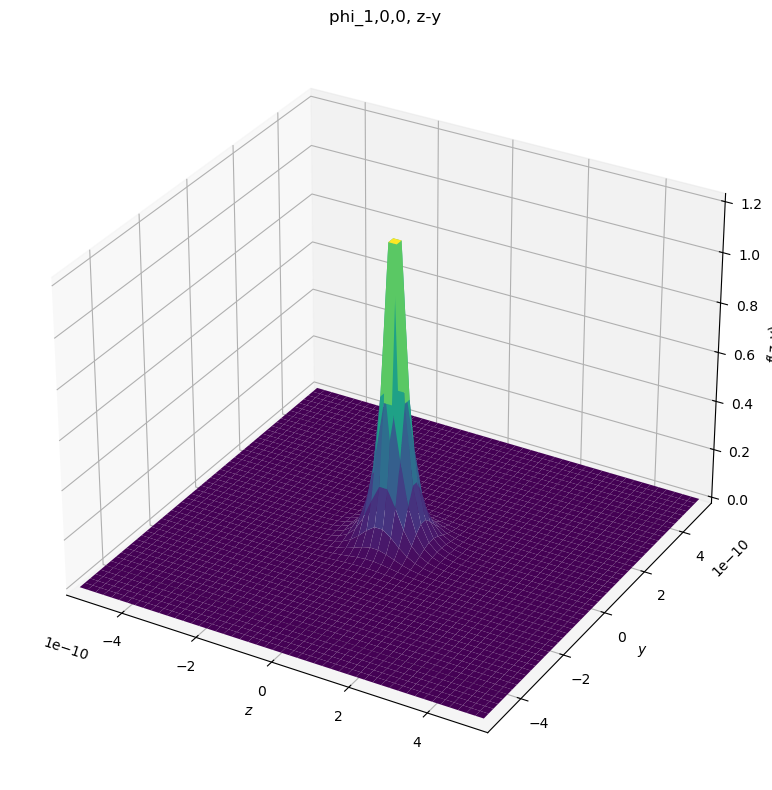
\includegraphics[width=0.7\textwidth]{1.1.png}
\end{figure}

\begin{figure}[H]
    \centering
    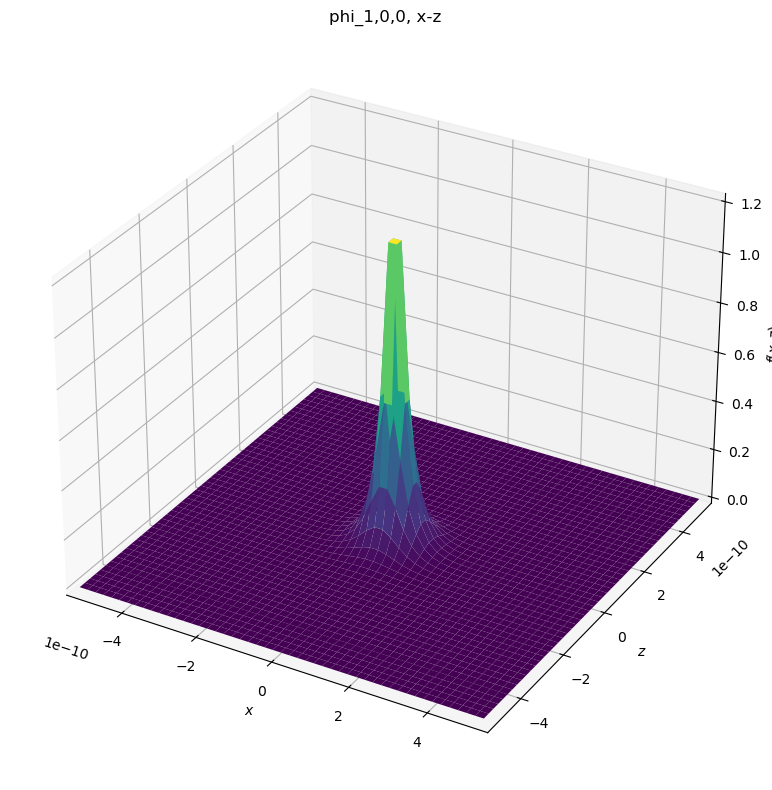
\includegraphics[width=0.7\textwidth]{1.2.png}
\end{figure}

\begin{figure}[H]
    \centering
    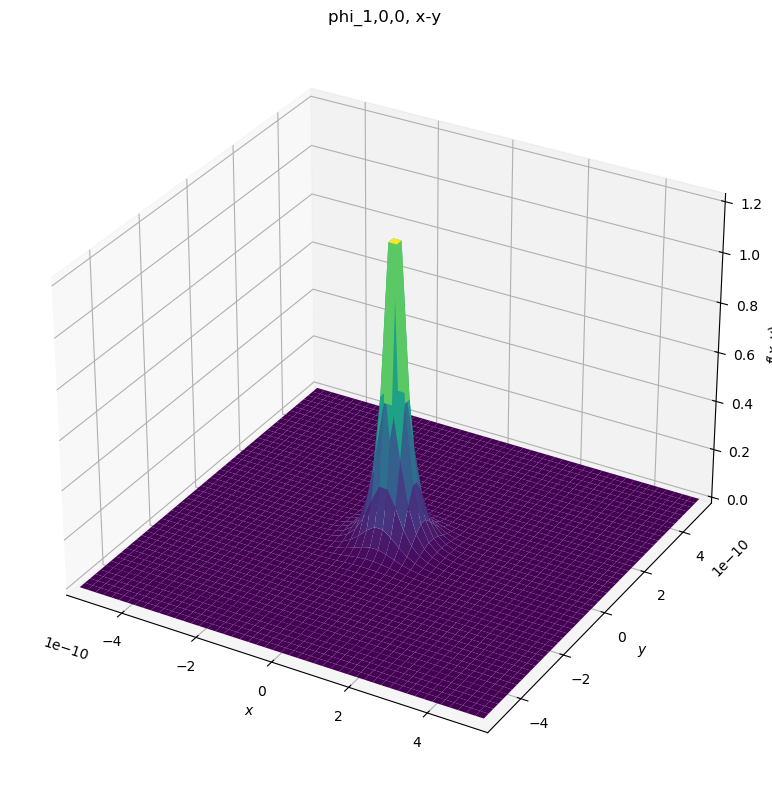
\includegraphics[width=0.7\textwidth]{1.3.png}
\end{figure}

\begin{figure}[H]
    \centering
    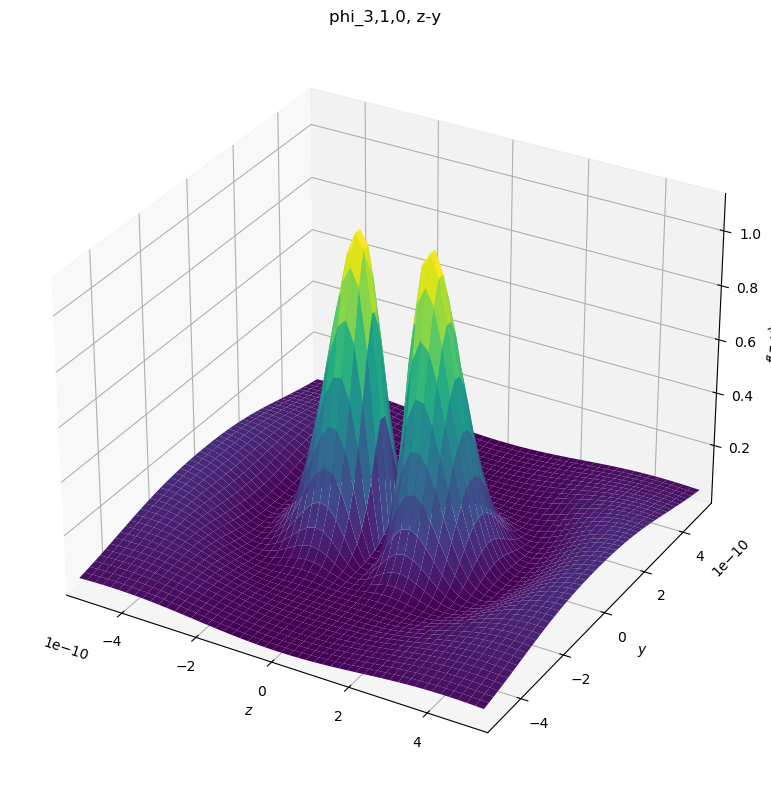
\includegraphics[width=0.7\textwidth]{3.1.png}
\end{figure}

\begin{figure}[H]
    \centering
    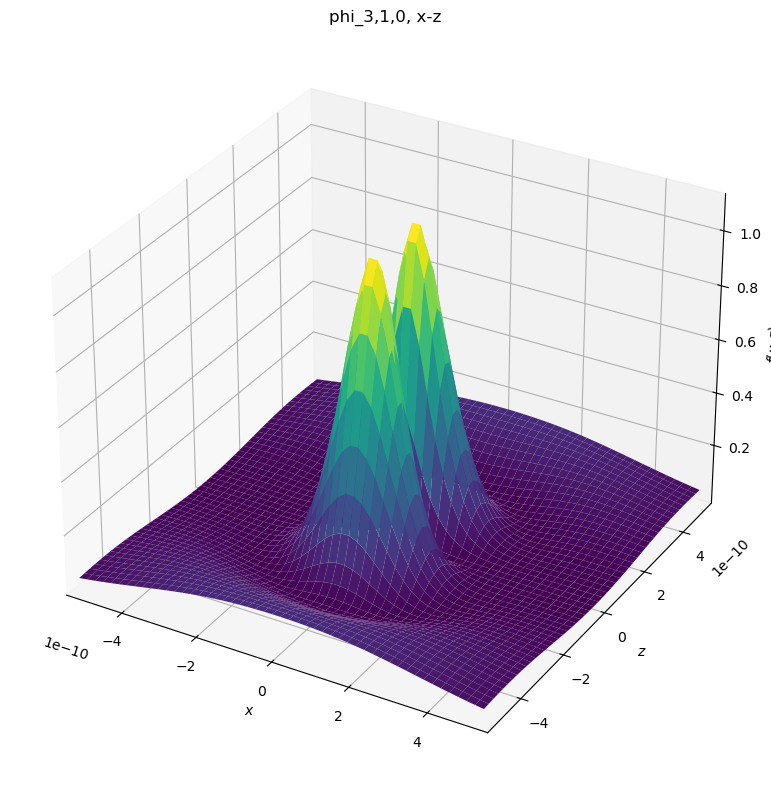
\includegraphics[width=0.7\textwidth]{3.2.png}
\end{figure}

Bei den anderen Plots werden leider Fehler generiert, weil im Ursprung Polarkoordinaten nicht wohl definiert sind.

\end{document}